\chapter{Multivariate Distributions}\index{multivariate distribution}

Taller people tend to weigh more. Students who sleep more tend to score higher. Snails with bigger shells tend
to be heavier. To describe two variables at once, including how they move together, you need a distribution
of two variables. In this chapter, you will meet the multivariate normal distribution, with real snail data,
and joint density functions, which use the double integrals you have just learned.

\section{Multivariate Distributions}
The world of probability and statistics does not limit itself to the
study of single variables. Often, we are interested in the
interconnections, relationships, and associations among several
variables. In such a scenario, the univariate distributions that we
have studied so far become inadequate. To comprehend the joint
behavior of these variables and to uncover the underlying patterns of
dependency, we must turn to the realm of multivariate distributions.

In this section, we look at the most important example: the
\index{multivariate distribution}multivariate normal distribution, along
with \index{covariance}covariance, which measures how two variables change
together.

\section{The Multivariate Normal Distribution}
Let us say that you are gathering statistics on a species of snail. You have found 89 snails.
Every snail has been weighed and had its shell measured. You have created a table like this:

\begin{tabular}{ c c }
Weight & Diameter \\
\hline
4.4769 grams & 2.2692 cm\\
5.4755 grams & 2.1973 cm\\
4.1183 grams & 2.52928 cm\\
... & ... \\
3.0522 grams & 1.7822 cm
\end{tabular}


You have been told that for any particular species of snail, the weight and shell diameter are typically normally distributed.
So, you compute the mean of each:

$$\bar{x} = \frac{\sum_{i=1}^{n} x_i}{n}$$

Your snails have a mean mass of 4.25 grams and a mean shell diameter of 2.35 centimeters.
Now you know where the center of each normal distribution will be.

To know how wide each normal distribution is, you need to compute the variance:

$$\sigma^2 = \frac{\sum_{i=1}^{n} (x_i - \bar{x})^2}{n}$$

(Reminder: The standard deviation is the square root of $\sigma^2$)

Plotting this data is shown in Figure~\ref{fig:pdfweight_diameter}.
\begin{figure}[H]
    \centering
    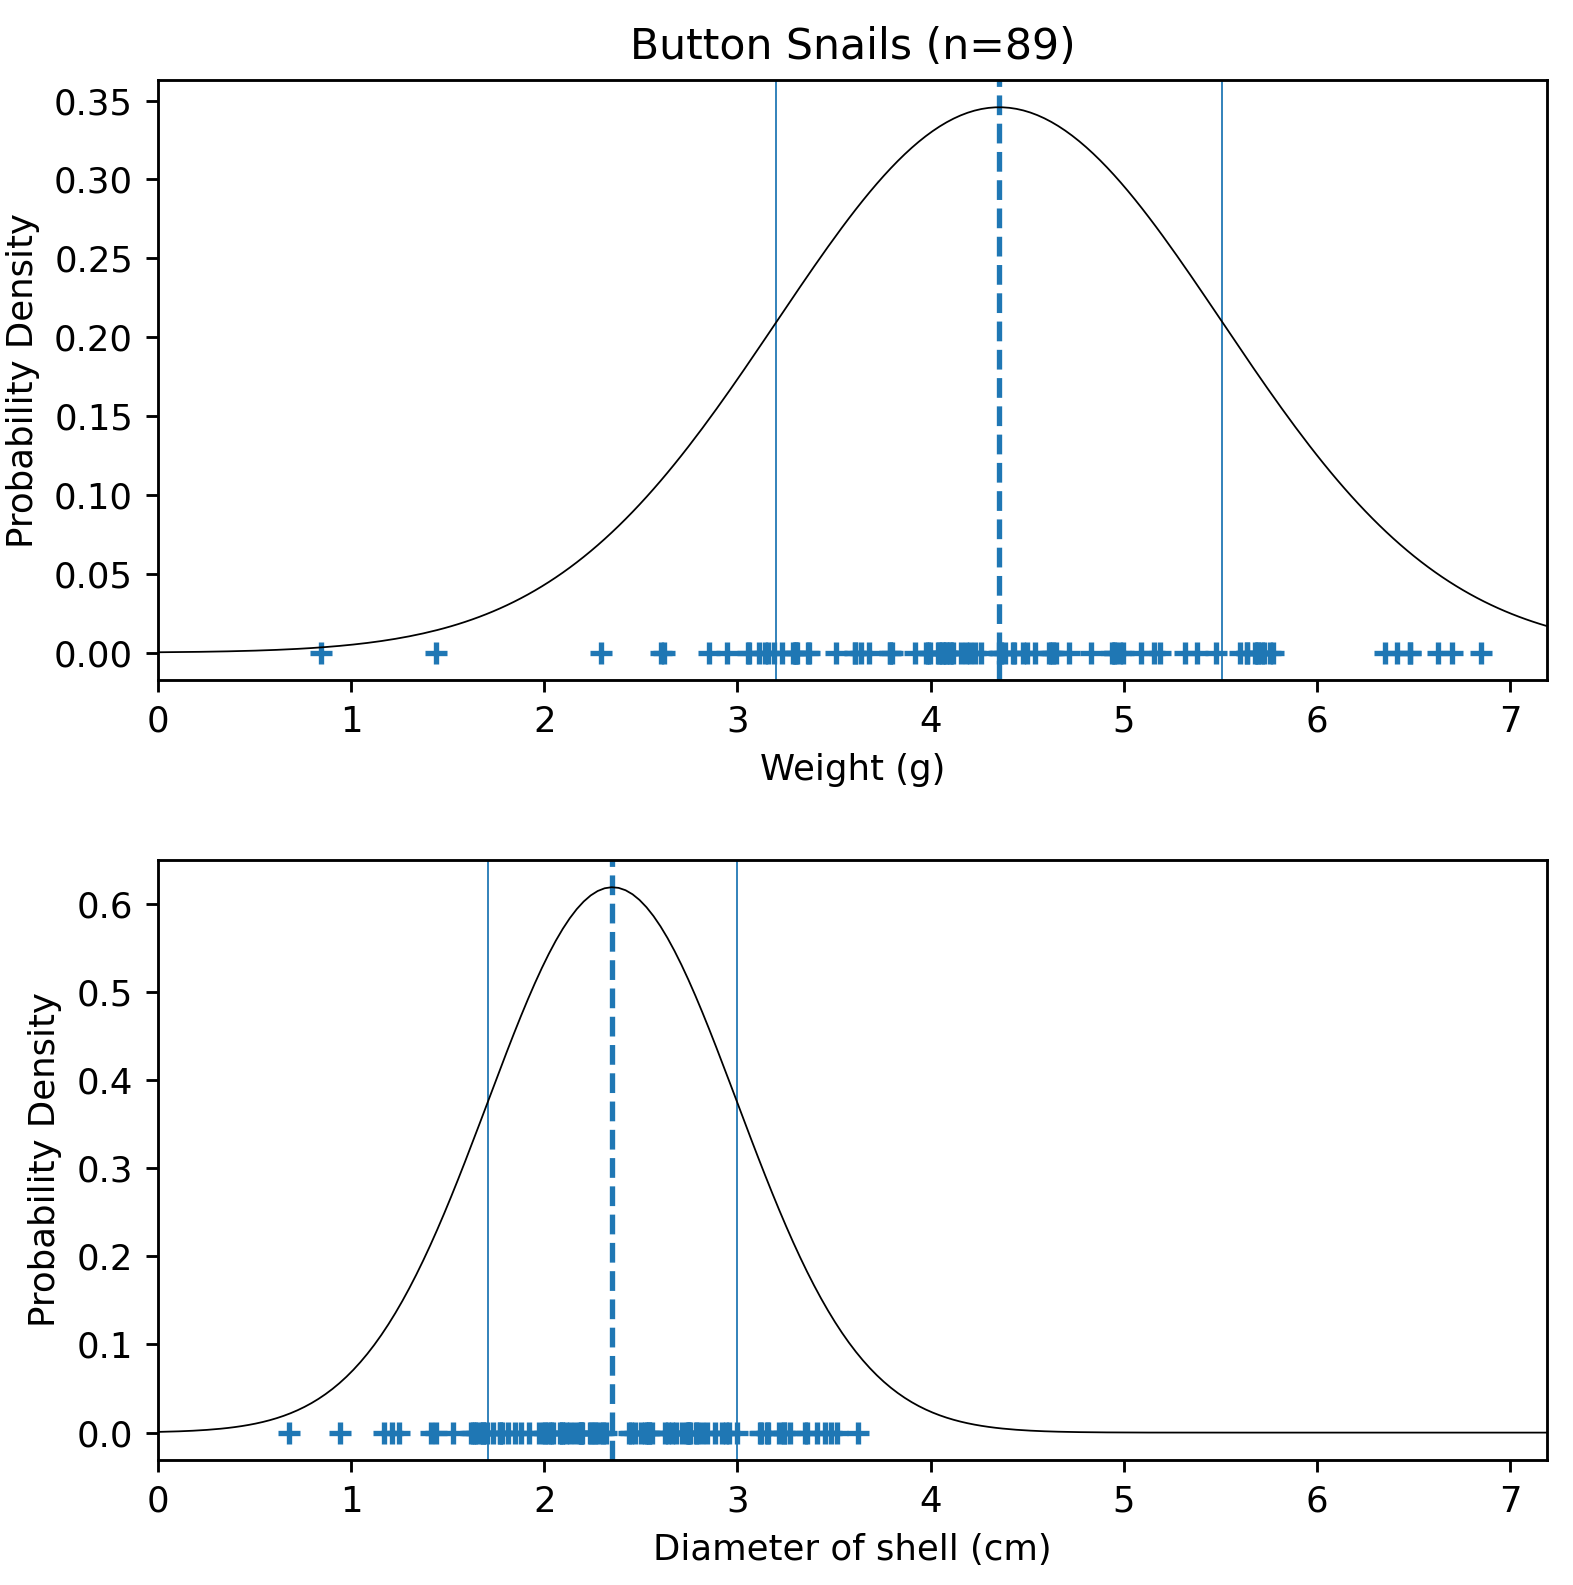
\includegraphics[width=0.55\textwidth]{separate.png}
    \caption{Probability density functions of weight and diameter.}
    \label{fig:pdfweight_diameter}
\end{figure}

Nice! However, then you think: "Hmm. Maybe the mass and the diameter of the shell are related. It seems like a heavy snail might tend to have a larger shell."  So, you make a scatter plot:

\begin{figure}[H]
    \centering
    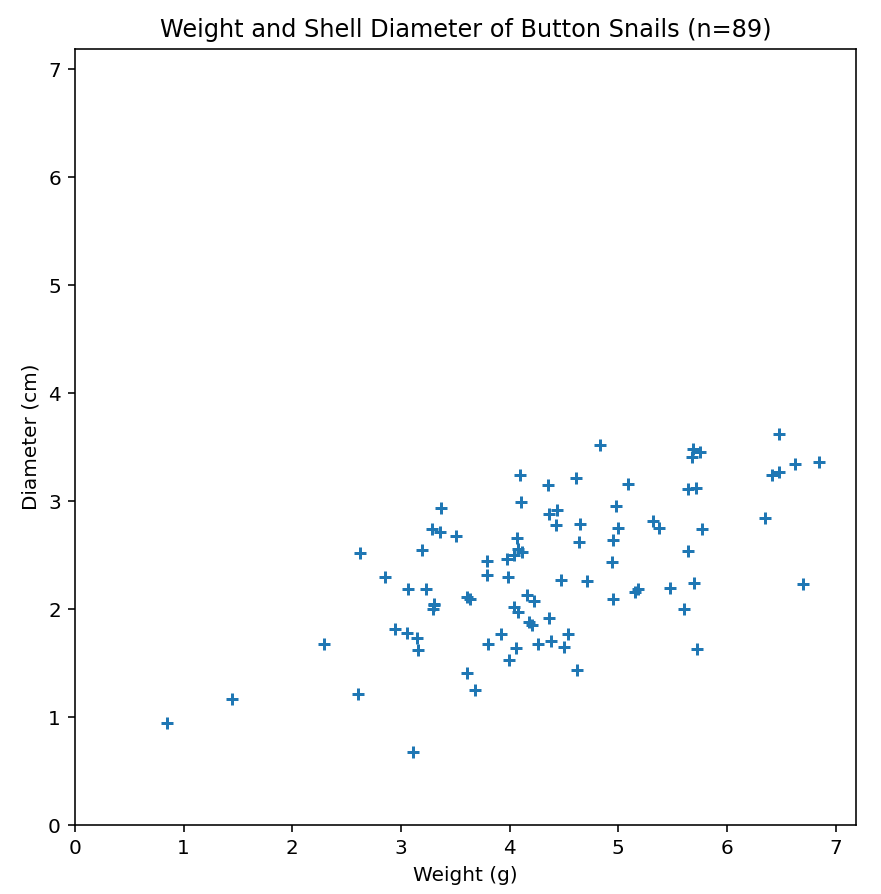
\includegraphics[width=0.55\textwidth]{scatter.png}
    \caption{A scatter plot with weight of the snail horizontally and diameter of the shell on the y-axis.}
    \label{fig:example_4}
\end{figure}

Sure enough, there is some \index{correlation}correlation between the mass of the snail and the diameter of its shell.

There is a form of the normal distribution that can deal with multiple variables and their correlations.
This is known as the \newterm{multivariate normal} (or multivariate Gaussian) distribution. \index{multivariate normal distribution} \index{Gaussian distribution}

In a multivariate normal distribution, the \index{mean vector}mean (often denoted $\boldsymbol\mu$) is a vector containing the mean of every variable.
For your snails, $\boldsymbol\mu = \begin{bmatrix} 4.25, 2.35 \end{bmatrix}$.

Just as in the single-variable normal distribution, measurements near the mean are what you are most likely to observe.
In a single-variable normal distribution, the standard deviation tells us how fast that likelihood falls off as we move away from the mean.
In multivariate normal distributions, we need something a little more expressive: a matrix.

\subsection{The Covariance Matrix}

We can think of the data as a list of vectors.
For example, if we have $n$ snails and $d$ properties that we have measured, we would get a list like this:

$$\begin{bmatrix}
x_{1,1} & x_{1,2} & ... & x_{1,d} \\
x_{2,1} & x_{2,2} & ... & x_{2,d} \\
... & ... & &... \\
x_{n,1} & x_{n,2} & ... & x_{n,d}\end{bmatrix}$$

Each row represents one snail. Each column represents one property.

Note that to make $\boldsymbol\mu$ (the mean vector), you just take the mean of each column of this data matrix. (For convenience, we will use $\boldsymbol\mu_i$ to refer to the mean of column $i$.)

We usually use $\mathbf{\Sigma}$ (the uppercase Greek sigma) to represent a \index{covariance matrix}covariance matrix. $\mathbf{\Sigma}$ is a $d \times d$ matrix.
The entries on the diagonal of $\mathbf{\Sigma}$ are just the variance of each property.
So, we can calculate the entry at row $j$, column $j$ like this:

$$\mathbf{\Sigma}_{j,j} = \frac{\sum_{i=1}^{n}(x_{i,j} - \boldsymbol\mu_j)^2}{n}$$

(Yes, we are using $\mathbf{\Sigma}$ to represent both summation and the covariance matrix here.
It can be confusing, but you will be able to tell from context how it is being used.)

The other entries, $\Sigma_{j,k}$ where $j \neq k$, are the \newterm{covariance} between property $j$ and property $k$.
If the covariance is a positive number, property $j$ and property $k$ are correlated. For example, in your snails, weight and diameter have a positive covariance: If the snail is heavier than average, it tends to have a diameter that is larger than average.

If the covariance is a negative number, when property $j$ is greater than average, property $k$ tends to be less than average.
For example, the number of times a restaurant mops the floor in a week has a negative covariance with how much bacteria lives on the floor.

How do we compute the \index{covariance!formula}covariance?

$$\mathbf{\Sigma}_{j,k} = \frac{\sum_{i=1}^{n}(x_{i,j} - \boldsymbol\mu_j)(x_{i,k} - \boldsymbol\mu_k)}{n}$$

Note that $\mathbf{\Sigma}_{j,k} = \mathbf{\Sigma}_{k,j}$, so the matrix is symmetric.

\subsubsection{Computing Mean and Covariance in Python}

If you have a numpy array where each row represents one sample and each column represents one property, it is really easy to compute $\boldsymbol\mu$ and $\mathbf{\Sigma}$:

\begin{minted}{python}
# Read in the data matrix, each row represents one snail
snails = ...

# Compute mu
mean_vector = snails.mean(axis=0)
print(f"Mean = {mean_vector}")

# Compute Sigma
covariance_matrix = np.cov(snails, rowvar=False)
print(f"Covariance = {covariance_matrix}")
\end{minted}

\subsection{Multivariate Normal Probability Density}

Now that we have good estimates of $\boldsymbol\mu$ and $\mathbf{\Sigma}$, how can we compute the probability density?

When you were working with just one variable, $x$, you computed the probability density using the mean $\mu$ and the variance $\sigma^2$ like this:

\begin{equation*}
p(x) = \frac{1}{\sqrt{2\pi\sigma^2}} e^{-\frac{(x - \mu)^2}{2\sigma^2}}
\end{equation*}

The probability density function of a $d$-dimensional
multivariate normal distribution with a mean of $\boldsymbol\mu$ and a covariance matrix of $\mathbf{\Sigma}$ is given by:

\begin{equation*}
p(\mathbf{x}) = \frac{1}{\sqrt{(2\pi)^d|\mathbf{\Sigma}|}}\exp\left(-\frac{1}{2}(\mathbf{x}-\boldsymbol\mu)^T\mathbf{\Sigma}^{-1}(\mathbf{x}-\boldsymbol\mu)\right)
\end{equation*}

If we draw lines to show where $\boldsymbol\mu$ is and contours to show lines of equal probability density, we get a plot shown in Figure~\ref{fig:contour_snail}.
\begin{figure}[H]
    \centering
    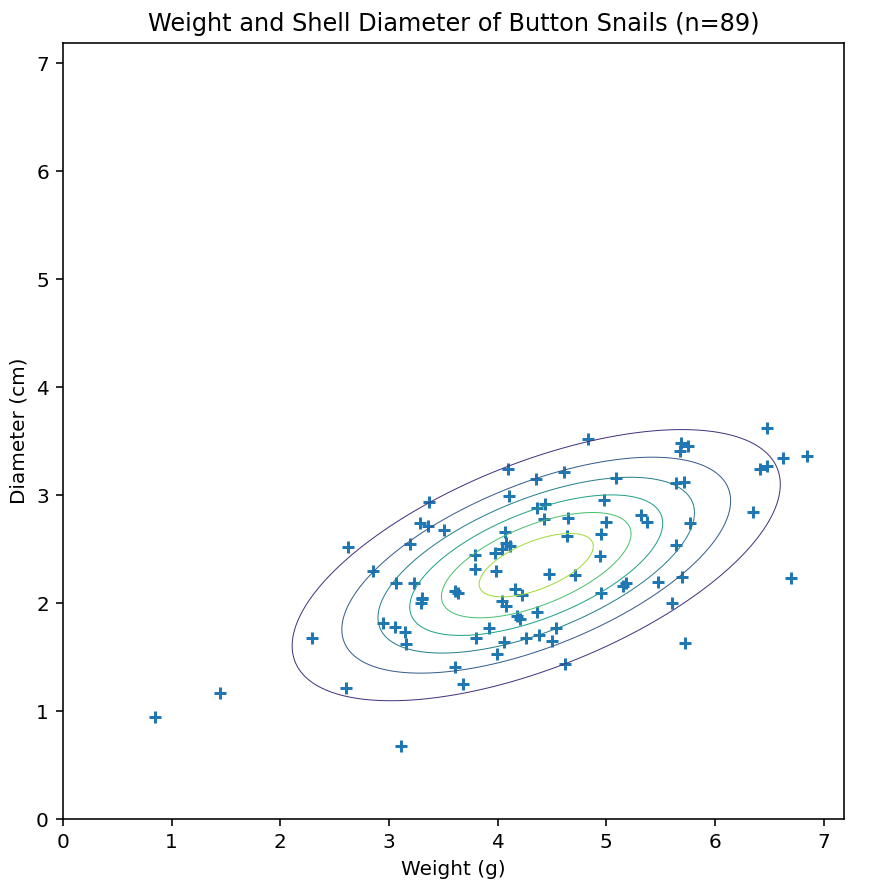
\includegraphics[width=0.55\textwidth]{contour.png}
    \caption{Contour plot of the snail data.}
    \label{fig:contour_snail}
\end{figure}

Or, we can do a 3D plot, as shown in Figure~\ref{fig:3d_snail}.
\begin{figure}[H]
    \centering
    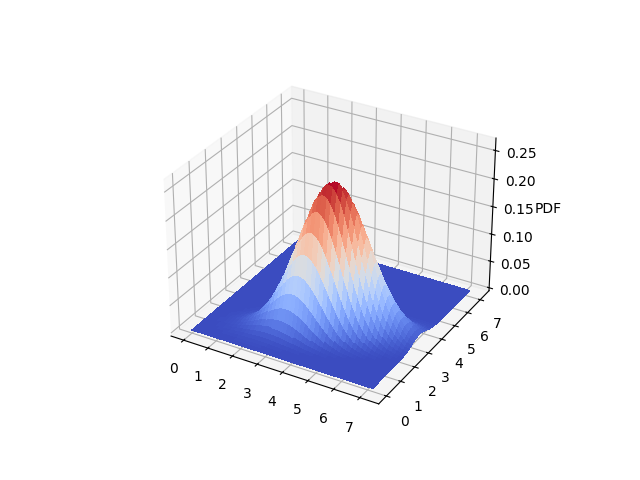
\includegraphics[width=0.55\textwidth]{3d.png}
    \caption{3D plot of the probability density function.}
    \label{fig:3d_snail}
\end{figure}

A probability density always integrates to 1.0, so the volume under the surface must be 1.0.

\subsubsection{Multivariate Normal Probability Density in Python}\index{multivariate normal!probability density}

The scipy library has a class that represents the multivariate normal. Here is how you could compute the probability density for a particular snail:

\begin{minted}{python}
import numpy as np
from scipy.stats import multivariate_normal

...Compute mean_vector and covariance_matrix...

# Get the probability density at [3 grams, 2 cm]
x = np.array([3.0, 2.0])
pd = multivariate_normal.pdf(x, mean=mean_vector, cov=covariance_matrix)
print(f"The probability density at {x} is {pd}")
\end{minted}

Alternatively, maybe you would like to generate weights and diameters for a fictional population of 700 snails:

\begin{minted}{python}
new_snails = multivariate_normal.rvs(mean=mean_vector, cov=covariance_matrix, size=700)
print(f"My fictional snails:\n{new_snails}")
\end{minted}

\section{Joint Density Functions}
Recall that you have learned about \textit{probability density functions} in a 
previous chapter. For some variable, $X$, with probability density function 
$f(x)$, the likelihood that $X$ lies between $a$ and $b$ is given by:
$$P(a \leq X \leq b) = \int_a^b f(x)\,dx$$

We can extend this to two random variables, $X$ and $Y$. A function that 
describes the distribution of both variables is called a \textit{joint 
density function}\index{joint density function}. In particular, the probability
that $X$ and $Y$ lie in a region $D$ is:
$$P((X, Y) \in D) = \iint_{\textit{D}} f(x,y)\,dA$$

Where $f(x, y)$ is the two-variable joint density function. Just like with one 
variable, all probabilities are positive and the sum of the probabilities of 
all possibilities must be 1. Mathematically, 
$$f(x, y) \geq 0$$
$$\iint_{\mathbb{R}} f(x, y)\,dA = \int_{-\infty}^{\infty} \int_{-\infty}^{
\infty} f(x, y)\,dx\,dy = 1$$

\textbf{Example}: Suppose the joint density function for $X$ and $Y$ is given 
by:
$$f(x, y) = 
\begin{cases}
C(3x + y),& \text{if }0 \leq x \leq 15\text{, }0 \leq y \leq 15\\
0,&\text{otherwise}
\end{cases}
$$

where $C$ is a constant. Find the value of $C$ and the likelihood that $X \geq 
Y$.

\textbf{Solution}: To find $C$, we take advantage of the fact that the sum of 
all probabilities is 1. Therefore,
$$1 = \int_0^{15} \int_0^{15} C(3x + y)\,dx\,dy = \int_0^{15} C \left[ \frac{3
}{2}x^2 + xy \right]_{x = 0}^{x = 15}\,dy$$
$$= \int_0^{15} C \left[ \frac{675}{2} + 15y \right]\,dy = C \left[ \frac{675}{
2}y + \frac{15}{2}y^2 \right]_{y = 0}^{y = 15}$$
$$= C \left[ \frac{10125}{2} + \frac{3375}{2} \right] = 6750C = 1$$

Which implies that $C = \frac{1}{6750}$.

To find the probability that $X \geq Y$, we note that this is represented by 
the region $R = \{(x, y)\text{ }|\text{ }0 \leq x \leq 15, 0 \leq y \leq x$. 
Then the likelihood that $X \geq Y$ is given by:
$$\frac{1}{6750} \int_0^{15} \int_0^x \left( 3x + y \right) \,dy\,dx = \frac{
1}{6750} \int_0^{15} \left[ 3xy + \frac{1}{2}y^2 \right]_{y = 0}^{y = x}\,dx$$
$$= \frac{1}{6750} \int_0^{15} \left(3x^2 + \frac{1}{2}x^2 \right)\,dx = \frac{
1}{6750} \left( \frac{7}{2} \right) \int_0^{15} x^2\,dx$$
$$= \frac{7}{13500} \left( \frac{1}{3} \right) \left[x^3 \right]_{x = 0}^{x = 
15} = \frac{7}{13500} \left( \frac{1}{3} \right) 15^3 = \frac{7 \cdot 3375}{3 
\cdot 13500} = \frac{7}{12}$$

And this answer makes sense, as it is less than 1. 

\begin{Exercise}[title = {Joint Density Functions}, label = joint]
The joint density function for a pair of random variables, $X$ and $Y$ is
$$f(x, y) = 
\begin{cases}
	ky(1 + 2x),& \text{if } 0 \leq x \leq 1\text{, }0 \leq y \leq 2\\
	0,&\text{ otherwise}
\end{cases}$$
\begin{enumerate}
\item Find the value of the constant, k.
\item Find $P(X \leq \frac{1}{2}, Y \leq 1)$.
\item Find $P(X + Y \geq 1)$.
\end{enumerate}
\end{Exercise}

\begin{Answer}[ref = joint]
\begin{enumerate}
    \item $$1 = \int_0^1 \int_0^2 ky\left(1 + 2x \right)\,dy\,dx = k \left[ 
    \int_0^1 1 + 2x\,dx \right] \cdot \left[ \int_0^2 y \,dy \right]$$
    $$= k \left[ \left(x + x^2 \right)_{x = 0}^{x = 1} \right] \cdot \left[ 
    \frac{1}{2} \left( y^2 \right)_{y = 0}^{y = 2} \right] = k \left( 2 \right)
    \left( \frac{1}{2} \right) \left(4 \right) = 4k$$

    If $4k = 1$, then $k = 1/4$. 

    \item $$P(X \leq \frac{1}{2}, Y \leq 1) = \int_0^{1/2} \int_0^1 \frac{1}{4}
    y \left(1 + 2x \right)\,dy\,dx$$
    $$= \frac{1}{4} \left[ \int_0^{1/2} \left(1 + 2x \right)\,dx \right] \cdot 
    \left[ \int_0^1 y\,dy \right] = \frac{1}{4} \left[ \left(x + x^2 \right)_{
    x = 0}^{x = 1/2} \right] \cdot \left[ \frac{1}{2} \left(y^2 \right)_{y = 0}
    ^{y = 1} \right]$$
    $$= \frac{1}{4} \left( \frac{1}{2} + \frac{1}{4} \right) \left( \frac{1}{2}
    \right) \left( 1 \right) = \frac{3}{32}$$

    \item If $X + Y \geq 1$, then $1 - X \leq Y \leq 2$ and 
    $$P(X + Y \geq 1 ) = \int_0^1 \int_{1 - x}^2 \frac{1}{4} y \left(1 + 2x 
    \right)\,dy\,dx$$
    $$= \frac{1}{4} \int_0^1 \left(1 + 2x \right) \frac{1}{2} \left[y^2 \right]
    _{y = 1 - x}^{y = 2}\,dx = \frac{1}{8} \int_0^1 \left(1 + 2x \right) \left(
    2^2 - \left(1 - x \right)^2 \right)\,dx$$
    $$= \frac{1}{8} \int_0^1 \left(1 + 2x \right) \left(3 + 2x - x^2 \right)\,
    dx = \frac{1}{8} \int_0^1 3 + 8x + 3x^2 - 2x^3\,dx$$
    $$= \frac{1}{8} \left[ 3x + 4x^2 + x^3 - \frac{1}{2}x^4 \right]_{x = 0}^{x 
    = 1} = \frac{1}{8} \left[3 + 4 + 1 - \frac{1}{2} \right] = \frac{1}{8} 
    \cdot \frac{15}{2} = \frac{15}{16}$$
\end{enumerate}
\end{Answer}

Often, two variables are independent of each other. If both variables are 
random, the joint density function for the two variables is the product of the 
two individual probability distributions. For example, if the probability 
distribution of an individual's height, $H$, is given by $f_1(h)$ and the 
probability distribution of an individual's blood pressure, $B$, is given by 
$f_2(b)$, then the joint probability function for height and blood pressure is 
$$f(h, b) = f_1(h)f_2(b)$$

\textbf{Example}: Sally is spending the day at Six Flags Over Georgia and is 
looking forward to riding several roller coasters. The wait time for the Great 
American Scream machine, $X$, is modeled by density 
function
$$f_1(x) = 
\begin{cases}
0,&\text{ if } x < 0\\
\frac{1}{45}e^{-x/45},&\text{ if } x \geq 0
\end{cases}$$

And the wait time for the Georgia Scorcher, $Y$, is modeled by density function
$$f_2(y) = 
\begin{cases}
0,&\text{ if } y < 0\\
\frac{1}{30}e^{-y/30},&\text{ if } y \geq 0
\end{cases}$$

What is the probability that she spends less than 45 minutes total waiting for 
the two rides?

\textbf{Solution}: Since the variables are independent, the joint density 
function for both wait times is:
$$f(x, y) = f_1(x) f_2(y) = 
\begin{cases}
    \frac{1}{1350}e^{-x/45}e^{-y/30},& \text{ if } x \geq 0, y \geq 0\\
    0,&\text{ otherwise}
\end{cases}$$

We want to know the probability that $X + Y < 45$, which is represented by the 
region, $R$, shown below.

\begin{center}
   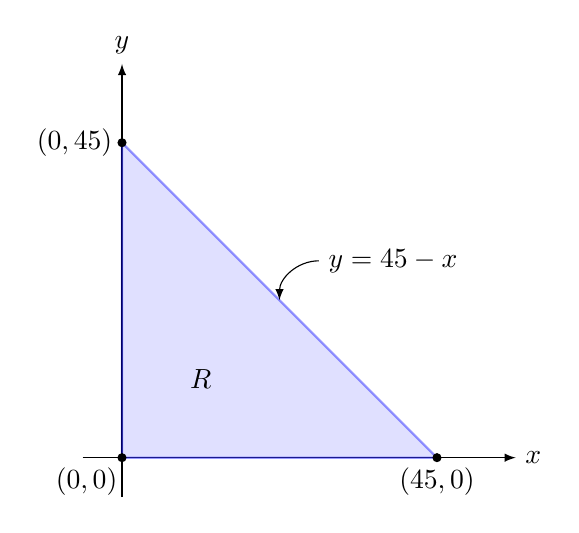
\begin{tikzpicture}
    \draw[-latex] (-0.5, 0) -- (5, 0) node[right] {$x$};
    \draw[-latex] (0, -0.5) -- (0, 5) node[above] {$y$};
    \draw[blue, thick, fill = blue!30, opacity = 0.4] (0,0) -- (0, 4) -- (4, 0)
     -- cycle;
    \draw[fill = black] (0,0) circle (0.05cm) node[below, xshift = -0.45cm] {
    $(0,0)$};
    \draw[fill = black] (4, 0) circle (0.05cm) node[below] {$(45, 0)$};
    \draw[fill = black] (0, 4) circle (0.05cm) node[left] {$(0, 45)$};
    \draw[latex-] (2, 2) arc [start angle = 180, end angle = 90, x radius = 
    0.5cm, y radius = 0.5cm] node[right] {$y = 45 - x$};
    \node[] at (1, 1) {$R$};
\end{tikzpicture}  
\end{center}

We can see that $R = \{(x, y)\text{ }|\text{ }0 \leq x \leq 45,\text{ }0 \leq 
y \leq 45 - x$. Therefore, the probability that Sally's total wait time is less
than 45 minutes is given by:
$$P(X + Y < 45) = \frac{1}{1350} \int_0^{45} \int_0^{45 - x} e^{-x/45} e^{-y/30
}\,dy\,dx$$
$$= \frac{-30}{1350} \int_0^{45} \left(e^{-x/45} \right) \left[e^{-y/30} 
\right]_{y = 0}^{y = 45 - x}\,dx$$
$$= -\frac{1}{45} \int_0^{45} \left( e^{-x/45} \right) \left[ e^{(x - 45)/30} 
- 1 \right]\,dx$$
$$= -\frac{1}{45} \int_0^{45} e^{(x - 135)/90} - e^{-x/45}\,dx$$
$$= -\frac{1}{45} \left[ 90e^{(x - 135)/90} + 45e^{-x/45} \right]_{x = 0}^{x = 
45}$$
$$= - \frac{1}{45} \left[ 90 \left( e^{(45 - 135)/90} - e^{(0 - 135)/90} 
\right) + 45 \left(e^{-45/45} - e^{-0/45} \right) \right]$$
$$= -\frac{1}{45} \left[90 \left( e^{-1} - e^{-3/2} \right) + 45 \left(e^{-1} 
- 1 \right) \right]$$
$$= -\frac{1}{45} \left[135e^{-1} - 90e^{-3/2} - 45 \right] = 1 + 2e^{-3/2} - 
3e^{-1} \approx 0.343$$

So, there is an approximately $34.3\%$ chance Sally will wait less than 45 
minutes to ride both roller coasters. 

\begin{Exercise}[title = {Snow Days}, label = snow]
In order for it to snow, two conditions must be met: the temperature must be 
low enough and the humidity must be high enough. The probability function for 
the temperature, $T$, in Celsius on a winter day is given by:
$$f_1(t) = 
\begin{cases}
    \frac{1}{80} \left[ \cos{\left( \frac{\pi t}{40} \right)} + 1 \right],& 
    -40 \leq t \leq 40\\
    0,&\text{otherwise}
\end{cases}
$$

And the probability function for the humidity, $H$, in percent on the same 
winter day is:
$$f_2(h) = 
\begin{cases}
    \frac{6(100h - h^2)}{1{,}000{,}000},& 0 \leq h \leq 100\\
    0,&\text{otherwise}
\end{cases}
$$

If the temperature must be below freezing and the humidity above 75\% for snow 
to form, what is the probability it snows?
\end{Exercise}

\begin{Answer}[ref = snow]
The humidity density must integrate to 1. Since $\int_0^{100}(100h - h^2)\,dh = 166{,}667$, the constant is $6/10^6$, so $f_2(h) = \frac{6(100h-h^2)}{10^6}$ on $0 \leq h \leq 100$. Because temperature and humidity are independent, the joint density is $f(t, h) = f_1(t)f_2(h)$.

The probability that snow forms is the product of the two separate probabilities:
$$P(T \leq 0, 75 \leq H \leq 100) = \left[\int_{-40}^{0} \frac{1}{80}\left(\cos{\frac{\pi t}{40}} + 1\right)\,dt\right]\left[\int_{75}^{100} \frac{6(100h - h^2)}{10^6}\,dh\right]$$

The first integral is $\frac{1}{80}\left[\frac{40}{\pi}\sin{\frac{\pi t}{40}} + t\right]_{-40}^{0} = \frac{1}{80}(40) = \frac{1}{2}$. The second is $\frac{6}{10^6}\left[50h^2 - \frac{h^3}{3}\right]_{75}^{100} = \frac{6}{10^6}\cdot\frac{78125}{3} = \frac{5}{32}$.

So $P = \frac{1}{2}\cdot\frac{5}{32} = \frac{5}{64} \approx 0.078$. There is about a 7.8\% chance it snows.
\end{Answer}
